\documentclass[conference]{IEEEtran}
%% VERSION 1.0
%% -----------------------------------------  (B) Packages
\usepackage[utf8]{inputenc}
\usepackage[english]{babel}
\usepackage{amsmath,amssymb,amsfonts}
\usepackage{algorithmic}
\usepackage{longtable}
\usepackage{adjustbox}
\usepackage{pdfpages}
\usepackage{hyperref}
\usepackage{graphicx}
\usepackage{textcomp}
\usepackage{csquotes}
\usepackage{booktabs}
\usepackage{siunitx}
\usepackage{xcolor}
\usepackage{array}
\usepackage{float}
\usepackage[citestyle=nature,bibstyle=nature]{biblatex}
%% -----------------------------------------  (E) Packages
%% -----------------------------------------  (B) Definitions
\def\BibTeX{{\rm B\kern-.05em{\sc i\kern-.025em b}\kern-.08em
    T\kern-.1667em\lower.7ex\hbox{E}\kern-.125emX}}
\addbibresource{bibliography.bib}
%% -----------------------------------------  (E) Definitions


\begin{document}
%% -----------------------------------------  (B) Header
\title{Stream Discharge and Stage Prediction with Machine Learning}

\author{\IEEEauthorblockN{Germán A. Jaramillo Ramírez, Ana C. Munguía Romero, Carlos N. Ojeda Angulo, Alejandro A. Bojorquez Pineda}
\IEEEauthorblockA{\textit{Escuela de Ingeniería y Ciencias, Campus Guadalajara} \\
\textit{Tecnológico de Monterrey}\\
Av. Gral. Ramón Corona No 2514, Colonia Nuevo México, Zapopan, Jalisco 45121,
México \\
a00571636@tec.mx, a01740019@tec.mx, a01741085@tec.mx, a01253099@tec.mx}}

\maketitle
%% -----------------------------------------  (E) Header
%% -----------------------------------------  (B) Metadata
%% \begin{abstract}
%%Aqui uno pone el abstract. puedes remover esta parte
%%\end{abstract}

% Aqui van las palabras clave. Se pueden remover desde begin a end y no pasa nada
\begin{IEEEkeywords}
Machine Learning, CNN, Regression, Stream Discharge, Stream Stage.
\end{IEEEkeywords}

%% -----------------------------------------  (B) Metadata
%% -----------------------------------------  (B) Introduction

\section{INTRODUCTION}
%para letras en negritas se usa \textbf{hola negritas}, para letras italicas \textit{italianoo} para cosas matematicas dentro del parrafo se ponen entre $3x =2$ y para cosas matematicas fuera de parrafo se pone $$xx+1=x3$$.

A streamgage contains instruments that measure and record the amount of water flowing in the river or stream, or its discharge \cite{streamgage}.

Having access to continuous data from streamgages is essential when calibrating and validating ground water and surface water models. Thus, encountering gaps in the data will increase uncertainty in the model predictions.

Cameras can help in this regard, since they provide redundancy with information unavailable from sensors. This imagery allows for hydrologic conditions to be visually verified (e.g., the presence of ice, obstructions, etc.).

In the instance of an actual gap in the data, having those images allows for
a qualitative assessment to confirm that the chosen gap filling method accurately represents the actual state of the stream during that certain time period.

With this, the objective of the current work is to fill stream discharge and stage data gaps using machine learning models for a location with camera availability.

The literature seems to support the notion of using cameras as a plausible way of insuring a sort of 'backup' of the data will be available in case of any technical failure of the sensors at the streamgage. Eltner, A. et al. (2021) show in their
research article \textit{Using Deep Learning for Automatic Water Stage Measurements} \cite{dl-waterstage} a similar use of deep learning tools as well as photogrammetric techniques to extract information from streamgage images to achieve more reliable water stage measurements. While the objective is most definitely not the same, the study sets a precedent for machine learning and image-based feature extraction applied to water monitoring.

\section{DATA DESCRIPTION}
Features were extracted from over 40,000 daylight images taken at one-hour intervals from 2012 to 2019. Dawn and dusk images that were too dark for feature extraction were removed.

The features were stored in a Comma Separated Value (CSV) file which contains the images’ names as ‘ Filename’ and, among many other features, the Stage and Discharge data from each image.

\section{METHODOLOGY}
\subsection{\textbf{Data storage}}
For a detailed explanation of the evolution and strategy for data management and storage, see \textit{Appendix B. Data Storage}.
\subsection{\textbf{Models generated with numeric data}}
\subsubsection{Data distribution}
The numeric data available in the CSV file is separated into three different datasets: testing, training and validation data.
These datasets were used when implementing the Multilayer Perceptron (MLP), Support Vector Regression (SVR) and Random Forest Regression (RFR) models for each of the dependent variables (stage and discharge).
\subsubsection{Recreating the original models}
The starting point of this work was to attempt to recreate the three models from the original research paper. Thus, the same ten features were used for the training stage: 'grayMean', 'graySigma', 'entropyMean', 'entropySigma', 'hMean', 'hSigma', 'sMean', 'sSigma', 'vMean', 'vSigma'.
\subsubsection{Principal Component Analysis (PCA)}
PCA was used for feature selection and new iterations of the models were trained with these variables.
\subsubsection{Preprocessing the data}
All of the above methods were alternatively trained with re-scaled data, using each of the following scalers: Standard, Robust and MinMax. Strings and non-numeric values have been dropped, except for the date, which was processed to create a new column called 'year' of numeric datatype.

\subsection{\textbf{Training Convolutional Neural Networks}}
We opted to make use of the already trained architectures \textit{EfficientNetB0} \& \textit{ResNet101} available in the \href{https://www.tensorflow.org/api_docs/python/tf/keras/applications}{\textit{Keras Applications} module}. We concluded that it'd be a better use of our time to focus on getting and comparing results rather than building an architecture from scratch, which, in the event of failure, we wouldn't really know if it failed due to errors
in the implementation or if it just wasn't the right fit for the project. Thus, we preferred to work with preexisting models that have already been proven to work in order to speed up the process.
\subsubsection{Data distribution}
The images were separated into two datasets: training and testing data. The images of each dataset were selected by years (2015-17 for testing and the remaining years for training), this due to the seasonal behaviour exhibited by the data.
\subsubsection{Preprocessing the data}
The images provided were of really good quality and of really big size, so resizing them was necessary in the code to ensure that the CNNs could receive them.
\subsubsection{EfficientNet}
Convolutional Neural Networks (CNN) tend to have fixed resources; this is quite a limitation since, conventionally, a CNN's depth or width would be increased as much as possible within the resource budget in an attempt to achieve greater accuracy rates. These are tedious and costly processes that may not always yield the desired outcome. EfficientNet proposes a new and more efficient method of scaling that scales all dimensions (depth, width and resolution) uniformly \cite{efficient-net}.
\subsubsection{ResNet}
The deeper the neural network, the harder it is to train. Due to their depth, they are able to start converging and that causes a degradation problem of training accuracy. This degradation indicates that not all systems are equally easy to optimize. As a way to ease the fitting of networks, the ResNet framework reformulates the layers of the network as learning residual functions with reference to the layer inputs, instead of having to learn unreferenced functions \cite{res-net}.
\subsubsection{Scope of the model}
Both \textit{ResNet101} and \textit{EfficientNetB0} take an incredibly long time to train (6 and 8 hours, respectively), and according to Hafeez, U. U. \& Gandhi, A. (2020) \cite{compute-times} execution times for CNN architectures are very costly and take up too many resources, even with the computational power of AWS. So it was decided to just train models to predict stream stage since the stage and discharge features are very highly correlated (making it possible to predict discharge with stage).

\subsection{\textbf{Loss metrics}}
The loss metrics (MAE, MSE, RMSE \& SE) used to evaluate the models were selected from the original paper so that we would have a way to effectively compare the results of this study with those obtained previously by the University of Nebraska.

\section{RESULTS}
\subsection{\textbf{Regression models}}
The regression models (MLP, RFR \& SVR) trained with the numeric data extracted from the images as provided in the CSV file were overall more reliable predicting stage rather than discharge.

Tables I through VI showcase the results of each iteration of every regression model worked on in this study.

While most models were inaccurate predicting stream discharge, the Random Forest Regression using robust scaling surpassed them by a lot with an $R^2$ value of $0.831$; error metrics, on the other hand, were pretty high all across the board and the RFR model got the lowest values of $MAE = 203.346$, $MSE = 232971.927$, $RMSE = 482.672$, $SE = 483.986$ (see \textit{Table II}).

%tables!
\begin{table}[H]
    \centering
    \caption{Discharge MLP}
    \begin{adjustbox}{width=\columnwidth,center}
    \begin{tabular}{llllll}
        ~ & MAE & MSE & RMSE & R\^2 & SE \\ \hline
        Normal* & 821.795 & 1383311.929 & 1176.143 & -0.001 & 1178.819 \\ 
        Normal (+ PCA)* & 678.002 & 1093322.927 & 1045.621 & 0.209 & 1046.412 \\ 
        Standard* & 365.059 & 475835.195 & 689.808 & 0.656 & 691.74 \\ 
        Standard (+ PCA) & 940.685 & 2261749.889 & 1503.912 & -0.637 & 1179.035 \\ 
        Robust*  & 362.85 & 459946.716 & 678.194 & 0.667 & 679.539 \\ 
        Robust (+ PCA) & 939.757 & 2259791.988 & 1503.26 & -0.636 & 1179.039 \\ 
        MinMax*  & 438.588 & 558835.307 & 747.553 & 0.595 & 746.6 \\ 
        MinMax (+ PCA) & 940.688 & 2261749.761 & 1503.911 & -0.637 & 1179.039 \\ 
        \bottomrule
        \multicolumn{6}{l}{\footnotesize *Normal: Raw data - unprocessed.}\\
        \multicolumn{6}{l}{\footnotesize *Standard: Standardly scaled data.}\\
        \multicolumn{6}{l}{\footnotesize *Robust: Robustly scaled data.}\\
        \multicolumn{6}{l}{\footnotesize *MinMax: MinMax Scaling applied to data.}\\
        \multicolumn{6}{l}{\footnotesize *(+ PCA): PCA run on the specified data.}\\
    \end{tabular}
    \end{adjustbox}
\end{table}

\begin{table}[H]
    \centering
    \caption{Discharge RFR}
    \begin{adjustbox}{width=\columnwidth,center}
    \begin{tabular}{llllll}
        ~ & MAE & MSE & RMSE & R\^2 & SE \\  \hline
        Normal* & 203.481 & 233258.04 & 482.968 & 0.831 & 484.288 \\ 
        Normal (+ PCA)* & 540.987 & 820620.085 & 905.881 & 0.406 & 908.206 \\ 
        Standard* & 203.365 & 233030.754 & 482.733 & 0.831 & 484.048 \\
        Standard (+ PCA) & 328.002 & 450925.772 & 671.51 & 0.674 & 673.313 \\ 
        Robust*  & 203.346 & 232971.927 & 482.672 & 0.831 & 483.986 \\ 
        Robust (+ PCA) & 549.581 & 912066.012 & 955.021 & 0.34 & 957.622 \\ 
        MinMax* & 203.43 & 233294.115 & 483.005 & 0.831 & 484.329 \\ 
        MinMax (+ PCA) & 295.01 & 403544.252 & 635.251 & 0.708 & 637.103 \\ 
        \bottomrule
        \multicolumn{6}{l}{\footnotesize *Normal: Raw data - unprocessed.}\\
        \multicolumn{6}{l}{\footnotesize *Standard: Standardly scaled data.}\\
        \multicolumn{6}{l}{\footnotesize *Robust: Robustly scaled data.}\\
        \multicolumn{6}{l}{\footnotesize *MinMax: MinMax Scaling applied to data.}\\
        \multicolumn{6}{l}{\footnotesize *(+ PCA): PCA run on the specified data.}\\
    \end{tabular}
    \end{adjustbox}
\end{table}

\begin{table}[H]
    \caption{Discharge SVR}
    \begin{adjustbox}{width=\columnwidth,center}
    \centering
    \begin{tabular}{llllll}
        ~ & MAE & MSE & RMSE & R\^2 & SE \\ \hline
        Normal* & 496.4 & 1069794.83 & 1034.309 & 0.226 & 995.413 \\ 
        Normal (+ PCA)* & 631.762 & 1249238.979 & 1117.694 & 0.096 & 1071.32 \\ 
        Standard* & 496.4 & 1069794.83 & 1034.309 & 0.226 & 995.413 \\ 
        Standard (+ PCA) & 489.712 & 1047283.417 & 1023.369 & 0.242 & 990.208 \\ 
        Robust*  & 496.4 & 1069794.83 & 1034.309 & 0.226 & 995.413 \\ 
        Robust (+ PCA) & 751.152 & 1515365.725 & 1231.002 & -0.097 & 1125.931 \\ 
        MinMax*  & 496.4 & 1069794.83 & 1034.309 & 0.226 & 995.413 \\ 
        MinMax (+ PCA) & 476.003 & 999011.14 & 999.505 & 0.277 & 969.637 \\ 
        \bottomrule
        \multicolumn{6}{l}{\footnotesize *Normal: Raw data - unprocessed.}\\
        \multicolumn{6}{l}{\footnotesize *Standard: Standardly scaled data.}\\
        \multicolumn{6}{l}{\footnotesize *Robust: Robustly scaled data.}\\
        \multicolumn{6}{l}{\footnotesize *MinMax: MinMax Scaling applied to data.}\\
        \multicolumn{6}{l}{\footnotesize *(+ PCA): PCA run on the specified data.}\\
    \end{tabular}
    \end{adjustbox}
\end{table}

For predicting stream stage specifically, the RFR using standard scaling yielded the best results out of all the regression models, with an $R^2$ value of $0.874$, and overall error metrics measuring lower than $0.3$ with $MAE = 0.14$, $MSE = 0.08$, $RMSE = 0.284$, $SE = 0.284$ (see \textit{Table V}).

\begin{table}[H]
    \centering
    \caption{Stage MLP}
    \begin{adjustbox}{width=\columnwidth,center}
    \begin{tabular}{llllll}
        ~ & MAE & MSE & RMSE & R\^2 & SE \\ \hline
        Normal* & 0.638 & 0.639 & 0.799 & -0.001 & 0.802 \\ 
        Normal (+ PCA)* & 0.631 & 0.773 & 0.879 & -0.212 & 0.877 \\ 
        Standard* & 0.211 & 0.112 & 0.335 & 0.824 & 0.336 \\ 
        Standard (+ PCA) & 0.296 & 0.227 & 0.476 & 0.644 & 0.478 \\ 
        Robust*  & 0.271 & 0.22 & 0.469 & 0.655 & 0.464 \\ 
        Robust (+ PCA) & 0.633 & 0.635 & 0.797 & 0.004 & 0.8 \\ 
        MinMax* & 0.237 & 0.142 & 0.377 & 0.777 & 0.376 \\ 
        MinMax (+ PCA) & 0.265 & 0.196 & 0.443 & 0.692 & 0.445 \\ 
        \bottomrule
        \multicolumn{6}{l}{\footnotesize *Normal: Raw data - unprocessed.}\\
        \multicolumn{6}{l}{\footnotesize *Standard: Standardly scaled data.}\\
        \multicolumn{6}{l}{\footnotesize *Robust: Robustly scaled data.}\\
        \multicolumn{6}{l}{\footnotesize *MinMax: MinMax Scaling applied to data.}\\
        \multicolumn{6}{l}{\footnotesize *(+ PCA): PCA run on the specified data.}\\
    \end{tabular}
    \end{adjustbox}
\end{table}

\begin{table}[H]
    \centering
    \caption{Stage RFR}
    \begin{adjustbox}{width=\columnwidth,center}
    \begin{tabular}{llllll}
        ~ & MAE & MSE & RMSE & R\^2 & SE \\ \hline
        Normal* & 0.14 & 0.08 & 0.283 & 0.874 & 0.284 \\ 
        Normal (+ PCA)* & 0.408 & 0.36 & 0.6 & 0.435 & 0.602 \\ 
        Standard* & 0.14 & 0.08 & 0.284 & 0.874 & 0.284 \\ 
        Standard (+ PCA) & 0.234 & 0.169 & 0.411 & 0.735 & 0.412 \\ 
        Robust* & 0.14 & 0.08 & 0.284 & 0.874 & 0.285 \\ 
        Robust (+ PCA) & 0.418 & 0.407 & 0.638 & 0.361 & 0.64 \\ 
        MinMax* & 0.14 & 0.08 & 0.283 & 0.874 & 0.284 \\ 
        MinMax (+ PCA) & 0.21 & 0.141 & 0.375 & 0.779 & 0.376 \\
        \bottomrule
        \multicolumn{6}{l}{\footnotesize *Normal: Raw data - unprocessed.}\\
        \multicolumn{6}{l}{\footnotesize *Standard: Standardly scaled data.}\\
        \multicolumn{6}{l}{\footnotesize *Robust: Robustly scaled data.}\\
        \multicolumn{6}{l}{\footnotesize *MinMax: MinMax Scaling applied to data.}\\
        \multicolumn{6}{l}{\footnotesize *(+ PCA): PCA run on the specified data.}\\
    \end{tabular}
    \end{adjustbox}
\end{table}

\begin{table}[H]
    \centering
    \caption{Stage SVR}
    \begin{adjustbox}{width=\columnwidth,center}
    \begin{tabular}{llllll}
        ~ & MAE & MSE & RMSE & R\^2 & SE \\ \hline
        Normal* & 0.172 & 0.086 & 0.294 & 0.864 & 0.295 \\ 
        Normal (+ PCA)* & 0.458 & 0.461 & 0.679 & 0.277 & 0.677 \\ 
        Standard* & 0.172 & 0.086 & 0.294 & 0.864 & 0.295 \\ 
        Standard (+ PCA) & 0.256 & 0.185 & 0.43 & 0.71 & 0.43 \\ 
        Robust*  & 0.172 & 0.086 & 0.294 & 0.864 & 0.295 \\ 
        Robust (+ PCA) & 0.596 & 0.592 & 0.77 & 0.071 & 0.757 \\ 
        MinMax*  & 0.172 & 0.086 & 0.294 & 0.864 & 0.295 \\ 
        MinMax (+ PCA) & 0.231 & 0.161 & 0.402 & 0.747 & 0.402 \\ 
        \bottomrule
        \multicolumn{6}{l}{\footnotesize *Normal: Raw data - unprocessed.}\\
        \multicolumn{6}{l}{\footnotesize *Standard: Standardly scaled data.}\\
        \multicolumn{6}{l}{\footnotesize *Robust: Robustly scaled data.}\\
        \multicolumn{6}{l}{\footnotesize *MinMax: MinMax Scaling applied to data.}\\
        \multicolumn{6}{l}{\footnotesize *(+ PCA): PCA run on the specified data.}\\
    \end{tabular}
    \end{adjustbox}
\end{table}

\subsection{\textbf{CNN models}}
The resulting values (see \textit{Table VII}) might make it seem that \textit{EffientNetB0} is the better model, but looking at the graph (\textit{Figure 1}) reveals that \textit{ResNet101}'s performance is much better (\textit{EffientNetB0} has a lot of noise and is really just predicting an average of the samples).

\begin{table}[H]
    \centering
    \caption{Stage using CNN}
    \begin{tabular}{llll}
        ~ & MAE & MSE & RMSE \\ \hline
        Resnet101 & 0.821 & 0.678 & 0.823 \\ 
        EfficientNetB0 &  0.338 & 0.184 & 0.4290 \\
    \end{tabular}
\end{table}

\begin{figure}[h]
\centering
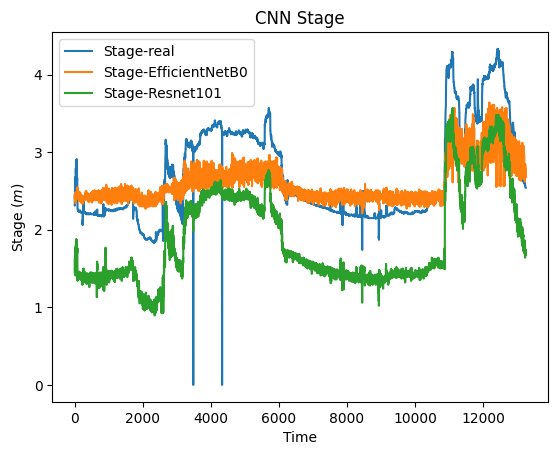
\includegraphics[width=0.4\textwidth]{CNN-Stage.png}
\caption{Comparison of models predicting stage}
\end{figure}

%% -----------------------------------------  (B) Discussion 
\section{DISCUSSIONS AND CONCLUSIONS}
In this project we proposed two different approaches: the first one using the variables from the CSV file with different scaling techniques and the second one using the 40,000+ images provided by the University of Nebraska to train preexisting CNN architectures.
The best results we got were from the Random Forest Regression model using standard scaling (for predicting stage) with a MSE of 0.08 and a MAE of 0.14, which seem to be good results, however, these values are not strictly an indicator of how reliable the model is, as it could be predicting an average of the samples instead of following the seasonal pattern or trend as it should be.

We believe that better results can be obtained if we continue working on CNNs while tweaking several different aspects that were not explored in this project, for example, grouping the data by week of the year, or month, to better take into account the seasonality of the data.

\newpage
\section{APPENDICES}

\subsection{Feature description}
\begin{table}[H]
\begin{center}
\begin{tabular}{|m{5em}|m{17em}|} 
 \hline
 \textbf{Header name} & \textbf{Description} \\ 
 \hline
 \textbf{Stage or Discharge} & \textbf{Response variables} \\ 
 \hline
 grayMean & Grey scale mean of all the pixel intensities after conversion from RGB to grey \\
 \hline
 graySigma & Grey scale sigma of all the pixel intensities after conversion from RGB to grey \\
 \hline
 entropyMean & Shannon entropy mean of all the gray scale pixel intensities after conversion from RGB to grey \\
 \hline
 entropySigma & Shannon entropy sigma of all the gray scale pixel intensities after conversion from RGB to grey \\
 \hline
 hMean & Mean of all the pixel intensities in the hue channel after conversion from RGB to HSV \\
 \hline
 hSigma & Sigma of all the pixel intensities in the hue channel after conversion from RGB to HSV \\
 \hline
 sMean & Mean of all the pixel intensities in the saturation channel after conversion from RGB to HSV \\
 \hline
 sSigma & Sigma of all the pixel intensities in the saturation channel after conversion from RGB to HSV \\
 \hline
 vMean & Mean of all the pixel intensities in the value channel after conversion from RGB to HSV \\
 \hline
 vSigma & Sigma of all the pixel intensities in the value channel after conversion from RGB to HSV \\  
 \hline
 grayMean 0 & Gray scale mean of all the pixel intensities in the above weir ROI \\
 \hline
 graySigma 0 & Gray scale sigma of all the pixel intensities in the above weir ROI \\
 \hline
 entropyMean 0 & Shannon entropy mean of all the gray scale pixel intensities in the above weir ROI \\
 \hline
 entropySigma 0 & Shannon entropy sigma of all the gray scale pixel intensities in the above weir ROI \\
 \hline
 hMean 0 & Mean of all the pixel intensities in the hue channel in the above weir ROI \\
 \hline
 hSigma 0 & Sigma of all the pixel intensities in the hue channel in the above weir ROI \\
 \hline
 sMean 0 & Mean of all the pixel intensities in the saturation channel in the above weir ROI \\
 \hline
 sSigma 0 & Sigma of all the pixel intensities in the saturation channel in the above weir ROI \\
 \hline
 vMean 0 & Mean of all the pixel intensities in the value channel in the above weir ROI \\
 \hline
 vSigma 0 & Sigma of all the pixel intensities in the value channel in the above weir ROI \\
 \hline
 grayMean 1 & Gray scale mean of all the pixel intensities in the below weir ROI \\
 \hline
 graySigma 1 & Gray scale sigma of all the pixel intensities in the below weir ROI \\
 \hline
 entropyMean 1 & Shannon entropy mean of all the gray scale pixel intensities in the below weir ROI \\
 \hline
 entropySigma 1 & Shannon entropy sigma of all the gray scale pixel intensities in the below weir ROI \\
 \hline
 hMean 1 & Mean of all the pixel intensities in the hue channel in the below weir ROI \\
 \hline
 hSigma 1 & Sigma of all the pixel intensities in the hue channel in the below weir ROI \\
 \hline
\end{tabular}
\end{center}
\end{table}

\begin{table}[H]
\begin{center}
\begin{tabular}{|m{5em}|m{17em}|} 
 \hline
 \textbf{Header name} & \textbf{Description} \\ 
 \hline
 sMean 1 & Mean of all the pixel intensities in the saturation channel in the below weir ROI \\
 \hline
 sSigma 1 & Sigma of all the pixel intensities in the saturation channel in the below weir ROI \\
 \hline
 vMean 1 & Mean of all the pixel intensities in the value channel in the below weir ROI \\
 \hline
 vSigma 1 & Sigma of all the pixel intensities in the value channel in the below weir ROI \\
 \hline
 WeirAngle & Angle of the weir \\
 \hline
 WeirPt1X & Far end of weir calculation end point X pixel position \\
 \hline
 WeirPt1Y & Far end of weir calculation end point Y pixel position \\
 \hline
 WeirPt2X & Near end of weir calculation end point X pixel position \\
 \hline
 WeirPt2Y & Near end of weir calculation end point Y pixel position \\
 \hline
 WwRaw LineMin & Minimum pixel distance from weir line to whitewater raw down stream edge \\
 \hline
 WwRaw LineMax & Maximum pixel distance from weir line to whitewater raw down stream edge \\
 \hline
 WwRaw LineMean & Mean of pixel distances from weir line to whitewater raw down stream edge \\
 \hline
 WwRaw LineSigma & Sigma of pixel distances from weir line to whitewater raw down stream edge \\
 \hline
 WwCurve LineMin & Minimum pixel distance from weir line to whitewater curve fit down stream edge \\
 \hline
 WwCurve LineMax & Maximum pixel distance from weir line to whitewater curve fit down stream edge \\
 \hline
 WwCurve LineMean & Mean of pixel distances from weir line to whitewater curve fit down stream edge \\
 \hline
 WwCurve LineSigma & Sigma of pixel distances from weir line to whitewater curve fit down stream edge \\
 \hline
\end{tabular}
\end{center}
\end{table}

\newpage
\onecolumn
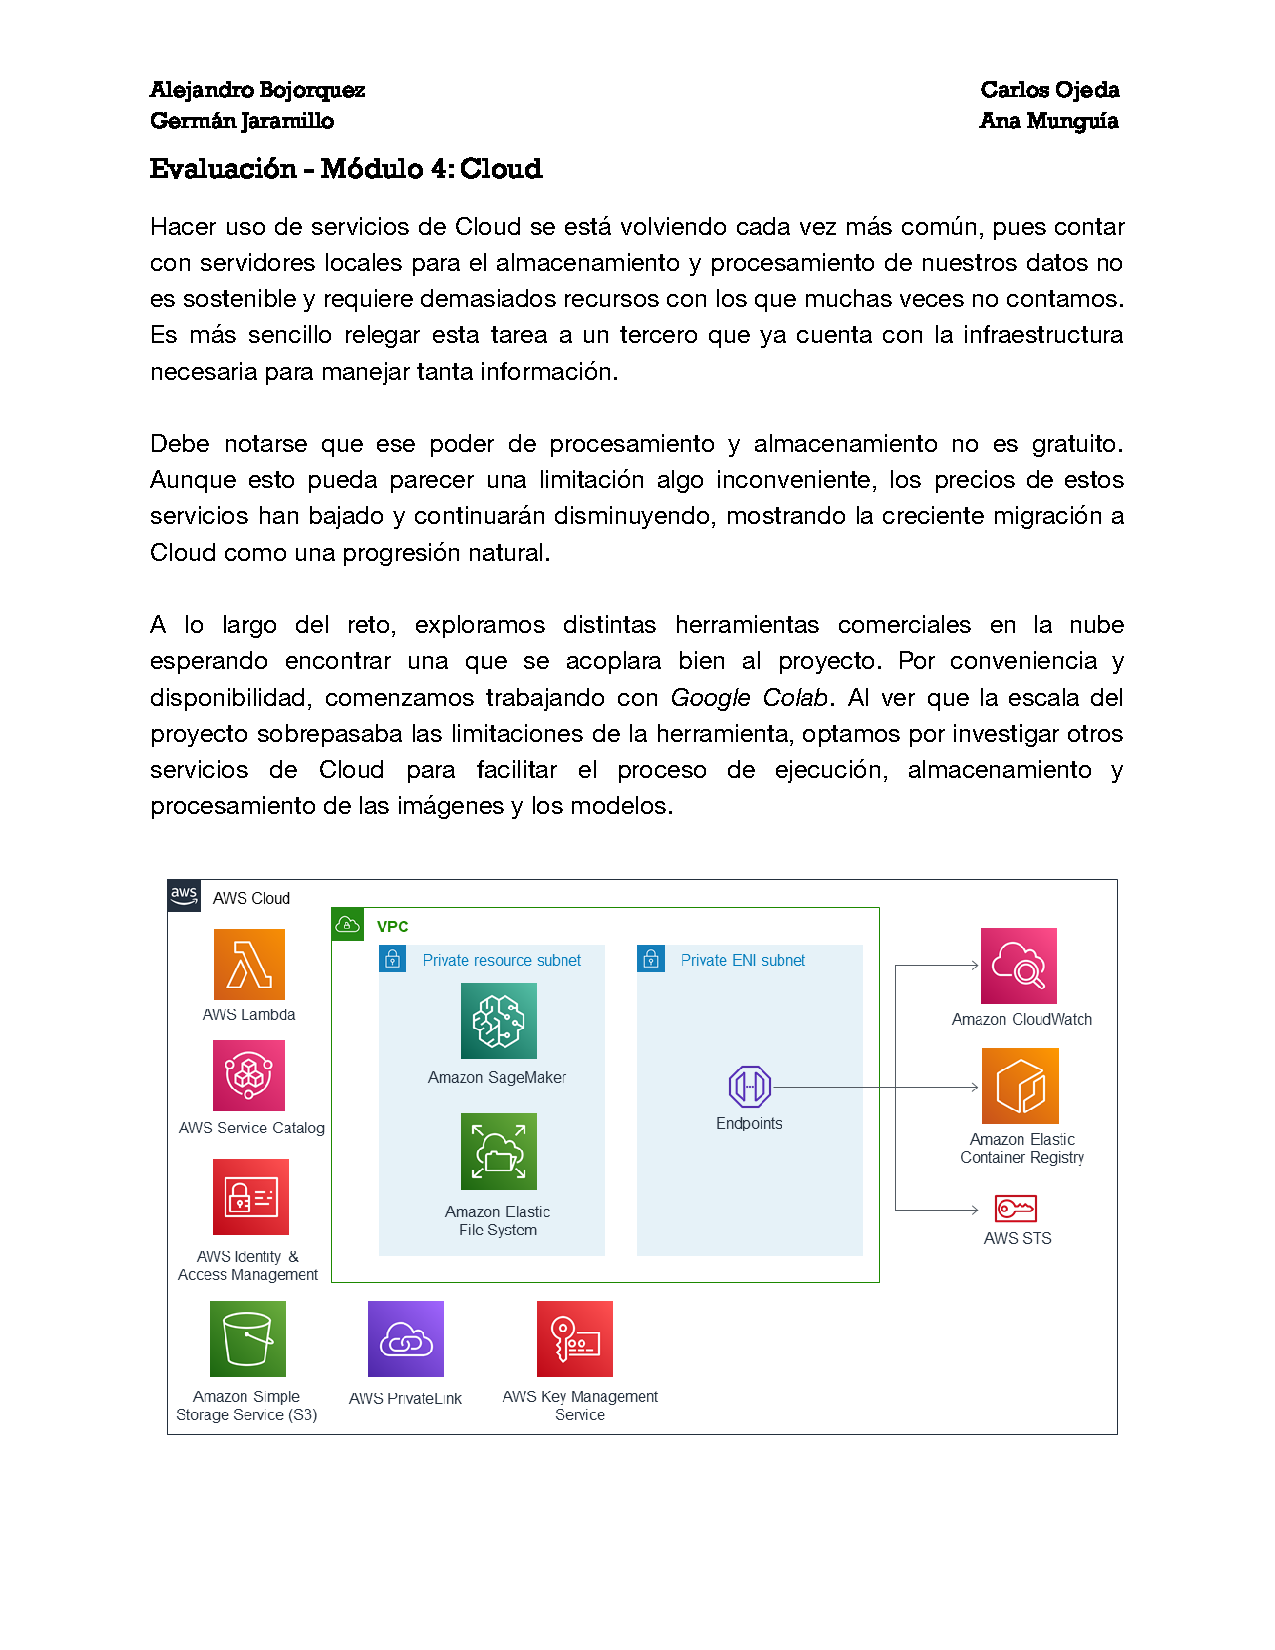
\includepdf[pagecommand={},scale=0.8,pages=1,pagecommand=\subsection{Data storage}
]{EvaluacionCloud.pdf}
\includepdf[scale=0.8,pagecommand={},pages=2-]{EvaluacionCloud.pdf}

\newpage
\twocolumn
\printbibliography
\end{document}